% Generated from 23-应用落地与商业化.md; edit the LaTeX source after migration.

\part*{第二十三部分 应用落地与商业化}
\addcontentsline{toc}{part}{第二十三部分 应用落地与商业化}
\markboth{第二十三部分 应用落地与商业化}{第二十三部分 应用落地与商业化}

技术路线能否成立，最终要回到场景。很多具身系统在实验室中都能展示能力，但只有少数能在特定场景中把能力、成本、稳定性和维护约束同时平衡出来。因此，本部分的重点不是重复场景分类，而是解释为什么某些场景更容易先跑通，以及商业化究竟被什么约束。这里最关键的判断标准不是“场景是否听起来足够宏大”，而是“场景是否允许局部结构化、是否能容忍有限失误、是否有足够高的价值密度去覆盖机器人系统成本”。

如果把应用落地问题抽象化，可以把单场景可行性理解为以下多因素函数：

\begingroup
\scriptsize
\begin{equation*}
\text{Viability} \approx f(\text{task structure}, \text{error tolerance}, \text{labor value}, \text{integration cost}, \text{maintenance burden})
\end{equation*}
\endgroup

这个表达式虽然不是严格商业模型，但足以说明一个现实：很多“技术上更炫”的场景，反而因为价值密度不足、误差容忍度太低或维护成本过高，而并不适合作为第一波商业化入口。

\chapter*{105. 制造业与仓储物流}
\addcontentsline{toc}{chapter}{105. 制造业与仓储物流}
\markboth{105. 制造业与仓储物流}{105. 制造业与仓储物流}

这仍然是当前最现实的落地方向之一。原因不是技术最简单，而是流程更容易局部结构化、ROI 更可量化、任务价值密度更高、现场维护体系更容易建立。也正因为如此，许多看起来“不够通用”的系统，反而更可能率先在这里形成真实价值。真正先跑出来的，通常不是“会做所有事”的机器人，而是能稳定接管某一类高频、高价值、可重复但又尚未被完全自动化的任务单元。仓储、分拣、搬运与工位协作也是 Agility、Amazon 等案例反复出现的主线。\href{https://agilityrobotics.com/}{Agility Robotics}、\href{https://www.aboutamazon.com/news/operations/amazon-tests-digit-humanoid-robot}{Amazon Robotics}

\section*{105.1 为什么这类场景总是反复领先}
\addcontentsline{toc}{section}{105.1 为什么这类场景总是反复领先}


制造、仓储、分拣与搬运场景之所以总是反复领先，并不是因为技术在这里最“先进”，而是因为它们最早满足了一组适合被交付的条件：任务可分解、价值密度高、收益可核算、失败可兜底、部署环境可被部分改造。也就是说，这类场景的优势不在于问题已经被彻底解决，而在于企业可以通过夹具、动线、工位约束、人工兜底和流程重组，把开放问题先压缩成一个可运营问题。

如果把场景落地能力抽象成一个粗略筛选式：

\begingroup
\scriptsize
\begin{equation*}
\text{Deployability} \propto
\frac{\text{task repetition} \times \text{value density} \times \text{verifiability}}
{\text{integration burden} \times \text{failure cost}},
\end{equation*}
\endgroup

那么制造与仓储的核心优势，通常不是分子绝对最大，而是分母更可控。它们允许企业逐步把复杂任务拆成高频、局部结构化的任务单元，只要系统能稳定接管其中一个高价值片段，就可能先形成真实商业收益。对商业化早期而言，这比一次性追求开放世界通用能力更重要。

更准确地说，这类场景长期领先的原因，是它们最适合做“运营压缩”：把原本散乱的感知、接触、恢复、验收和责任链，先压缩到一个客户能接受的范围内。只要企业能够把任务边界、异常处理、人工兜底和 ROI 计算稳定下来，它就在积累一种比单次模型性能更重要的能力，即“把机器人组织成可持续使用资产”的能力。

因此，本节最值得强调的判断不是“这些场景天然优质”，而是“这些场景最适合沉淀交付能力”。企业在这里真正建立的，往往不只是某个仓储或制造案例，而是一整套方法：如何定义任务单元、如何设计人工兜底、如何度量 ROI、如何把异常恢复流程写进运维模板、如何把单站点经验复制到第二个站点。这些能力一旦形成，才有可能外溢到更复杂场景。

从后续跟踪口径看，这类场景真正值得记录的也不是“又多了一个试点”，而是三类更硬的指标：第一，人工基线是否清楚，即原流程的人力、节拍和错误成本是否可量化；第二，机器人介入后是否把异常处理、夜班覆盖、危险工序或高波动工位稳定压下来；第三，第二站点复制时新增的工位改造、软件适配和运维负担是否明显下降。只有当这些指标持续改善时，制造与仓储场景的领先才不只是阶段性热度，而是交付组织能力的真实积累。

\section*{105.2 典型任务单元的判断标准}
\addcontentsline{toc}{section}{105.2 典型任务单元的判断标准}


任务单元判断之所以必须细到单元级，而不能停留在“行业/场景”级，是因为真正决定可商业化的往往不是整个行业是否需要机器人，而是某个具体工作片段是否足够结构化、是否容易度量收益、是否允许局部自动化先切入。仓储、制造、巡检、农业这些大类内部，往往同时包含适合早落地和暂不适合落地的子任务。

因此，任务单元的判断必须压到比“行业/场景”更细的层级。真正决定可商业化的，往往不是整个行业是否需要机器人，而是某个具体工作片段是否足够结构化、是否容易度量收益、是否允许局部自动化先切入。对制造与仓储场景，更有意义的不是泛泛说“机器人进工厂/仓库”，而是拆到搬运、上下料、分拣、包装、质检、巡检、工位协作这些最小闭环，再分别问它们需要什么感知、接触、时延与恢复能力。

把这套判断压缩成一个更工程化的筛选式，可以写成：

\begingroup
\scriptsize
\begin{equation*}
\text{TaskScore} =
w_1 \cdot \text{observability}
+ w_2 \cdot \text{repeatability}
+ w_3 \cdot \text{value density}
- w_4 \cdot \text{failure cost}
- w_5 \cdot \text{integration burden}
\end{equation*}
\endgroup

这当然不是为了制造一个可以机械打分的商业公式，而是提醒我们：一个任务单元之所以适合作为具身切入口，几乎从来都不是因为“模型已经足够强”这一条，而是因为观测、恢复、验收、付费和集成五个维度形成了相对有利的组合。很多演示看起来能做的任务，最后死在高失败代价和高集成摩擦；很多看起来不够性感的任务，则因为重复度高、收益明确而率先变成现实业务。

因此，后续评估任何任务单元时，最值得固定记录的问题只有五个：任务输入是否可感知，目标状态是否可验收，失败后是否存在低成本恢复路径，接入现有流程是否需要大规模改造，以及客户是否已经为该环节持续付钱。只有拆到这一层，本章才会真正成为商业判断工具，而不是对几个大行业的宏观赞美。

\chapter*{106. 家庭、消费级服务与医疗康复}
\addcontentsline{toc}{chapter}{106. 家庭、消费级服务与医疗康复}
\markboth{106. 家庭、消费级服务与医疗康复}{106. 家庭、消费级服务与医疗康复}

家庭和消费场景最接近“通用具身终局”，但短期最难规模化；医疗和康复则价值明确，但监管、责任和验证门槛极高。这两类场景都值得长期关注，但不应轻易被视为短期爆发主线。家庭场景最难的不是单个任务，而是开放度极高、语义模糊、对象多样、且任何失误都直接面向终端用户；医疗场景则最难在于即便技术能力不错，也必须先通过责任、流程和合规边界。

\section*{106.1 这两类场景为什么常被高估}
\addcontentsline{toc}{section}{106.1 这两类场景为什么常被高估}


家庭与医疗康复场景之所以常被高估，不是因为它们不重要，而是因为它们同时具备“高可见度”和“高终局想象力”。家庭直接连接大众生活，医疗康复直接连接高价值需求与社会善意，这使它们天然适合承载“未来生活方式改变”的叙事。但从部署角度看，这恰恰是两类最难被快速工程化的场景。

家庭场景的困难，在于开放环境、长尾物体、家庭成员干扰、儿童与宠物共处、长期售后和日常维护条件都远比工业现场复杂。医疗康复的困难，则在于责任链、伦理约束、流程嵌入、设备认证与人工接管边界必须同时成立。也就是说，这两类场景都不是“单次动作做出来”就能成立的场景，而是“整套责任体系和长期运维体系”必须共同成立的场景。

它们之所以被系统性高估，还有一个更隐蔽的原因：演示价值和商业价值在这里更容易被混写。家庭场景里，一个系统只要能在少数物体、少数房间、少数脚本中完成看起来“像生活”的任务，就足以获得极强传播效果；医疗康复里，只要机器人表现出对人体动作、护理流程或陪伴交互的某些片段能力，就会被天然赋予更高善意解读。但传播强化并不等于部署门槛下降。

因此，本章对它们采用“长期高价值、短期慢兑现”的判断口径。未来若出现声称在家庭或医疗康复场景取得突破的新系统，最值得优先核查的不是演示视频的流畅度，而是四类证据：开放环境鲁棒性、长期维护可行性、责任边界清晰度，以及真实用户条件下的长周期使用记录。只要这些证据还薄弱，就不应把它们直接写成短期主线。叙事强度在这里往往与短期可交付性反向相关，这是阅读相关新闻时最需要刻意校正的偏差。

更具体地说，家庭与医疗康复场景都存在一种“不可见人工被系统性低估”的问题。家庭产品往往需要复杂安装、远程客服、频繁地图重建与用户教育；医疗康复系统则更容易把医生、治疗师、护理员和合规团队的协作成本藏在机器人之外。若只看机器人本体动作是否完成，而不看这些外围组织成本，几乎必然会高估其商业成熟度。因此，这两类场景最该记录的不是单次演示完成率，而是“每次成功背后动用了多少额外人力、流程与责任兜底”。

\chapter*{107. 农业、建筑、巡检与危险环境}
\addcontentsline{toc}{chapter}{107. 农业、建筑、巡检与危险环境}
\markboth{107. 农业、建筑、巡检与危险环境}{107. 农业、建筑、巡检与危险环境}

这些场景的共同点，是环境复杂、人工成本高或危险性强，因此即使系统能力不完美，只要显著降低风险或节省成本，就可能具备商业价值。它们也经常更能容纳 shared autonomy 与远程接管路线。也就是说，这些场景对“完全自律”的执念反而更弱，对“显著降低风险”的要求更强。

\section*{107.1 为什么“半自主”在这些场景里更现实}
\addcontentsline{toc}{section}{107.1 为什么“半自主”在这些场景里更现实}


“半自主”更现实，并不是因为企业不想做全自主，而是因为农业、建筑、巡检和危险环境这类场景同时要求安全、责任可控、客户可接受和逐步上线。系统不一定要在所有条件下 100\% 独立完成任务，只要它能稳定接管最危险、最脏累、最耗时或最重复的那部分工作，就已经可能显著改善效率与安全。因此，shared autonomy 在很多时候不是过渡方案，而是商业最优方案。

如果把商业价值粗略写成

\begingroup
\scriptsize
\begin{equation*}
\text{Value} \approx
\text{autonomous coverage} \times \text{task value density}
- \text{handoff cost}
- \text{failure cost},
\end{equation*}
\endgroup

那么高风险复杂场景的关键，往往不是把 \texttt{\detokenize{autonomous coverage}} 推到 100\%，而是把高价值片段稳定接管，并把 \texttt{\detokenize{handoff cost}} 与 \texttt{\detokenize{failure cost}} 压到客户可以接受的范围内。Skydio 的工业巡检与公共安全产品线、以及 Boston Dynamics 的 Spot 方案，都长期把远程任务组织、现场运维和任务级自治作为产品形态的一部分，而不是把“完全无人化”当作唯一卖点。\href{https://www.skydio.com/}{Skydio} \href{https://bostondynamics.com/spot/}{Spot}

从系统组织方式看，半自主路线通常可以拆成三层责任分配。机器负责高频、危险或高体力负担片段；人类负责模糊决策、异常确认与责任兜底；运维系统负责监控、远程接入、任务切换和故障恢复。它的价值不在于“将就着只做一半”，而在于重新分配最稀缺的人类注意力，让人不再被迫持续占据低价值、高风险或高疲劳负担环节。

这类系统的最小调度逻辑甚至可以非常朴素：

\begin{lstlisting}[language=python]
while mission_active:
    state = robot.observe()
    if policy.confident(state):
        robot.execute(policy.act(state))
    else:
        handoff = remote_operator.resolve(state)
        robot.execute(handoff.action)
    logger.record(state, outcome)
\end{lstlisting}

真正决定商业成立与否的，不是这段逻辑是否优雅，而是 \texttt{\detokenize{policy.confident}} 的阈值如何设定、远程接管时延是否可控、单个操作员能覆盖多少台设备、异常恢复成本能否持续下降。也正因如此，分析这类场景时不应迷信“自主率越高越好”，而应优先看任务价值、接管成本与责任边界是否被组织成一个稳定闭环。

\chapter*{108. 商业模式}
\addcontentsline{toc}{chapter}{108. 商业模式}
\markboth{108. 商业模式}{108. 商业模式}

\section*{108.1 硬件销售}
\addcontentsline{toc}{section}{108.1 硬件销售}


硬件销售模式最容易被误读的一点，在于它表面上卖的是一台机器，实质上卖的是一整套可持续使用能力。只要系统仍然需要频繁校准、复杂维护、远程支持、版本兼容处理和异常兜底，那么“卖出去一台设备”背后就已经隐含了持续的服务责任。这意味着很多公司以为自己在走轻资产硬件路线，实际上却已经被运维和版本管理重新拖回系统公司逻辑。

因此，判断硬件销售是否成立，不能只看客户是否愿意为本体付费，更要看设备交付后的真实组织负担。若客户必须长期依赖原厂工程师驻场、每次升级都显著影响稳定性、关键零部件替换成本过高，或现场重新标定频率居高不下，那么所谓硬件销售很可能只是把后续服务成本隐藏到了合同之外。真正成熟的硬件销售，往往意味着设备、维护和升级边界已经足够清晰，以至于客户可以把它视为一类“可管理资产”，而不是“持续求助的实验系统”。

也正因为如此，研究型报告在看硬件销售时，不应只盯 ASP 或出货量，更应看安装周期、备件消耗、维护频次、版本兼容成本，以及软件升级是否会重新引入现场风险。具身行业里的“硬件销售”天然带有服务尾巴；区别只在于这条尾巴是被公司主动产品化了，还是被现实被动拖出来。

\section*{108.2 解决方案集成}
\addcontentsline{toc}{section}{108.2 解决方案集成}


解决方案集成模式之所以在具身领域反复出现，是因为它最适合吸收早期技术的不稳定性。与其要求机器人直接成为标准化产品，不如先把本体、工位改造、感知布局、夹具设计、软件接口和人工兜底一起打包成可交付方案。这样做虽然牺牲了部分标准化程度，却更容易在高价值客户现场率先形成闭环。对很多早期团队来说，这比直接卖通用机器人或押注远期平台化更现实。

但这条路线的风险也很明显：它容易把企业推入项目制泥潭。若每拿下一个客户都要重做大量定制开发、重新调夹具、重写接口和重建异常处理流程，那么收入虽然可以增长，能力却不一定真正沉淀。判断这一模式是否健康，关键要看公司是否在每轮项目交付中不断提炼出可复用模块、可复制流程和更稳定的任务模板，而不是只靠项目堆人。

解决方案集成路线还有一个经常被低估的价值：它是把隐性场景知识重新编码进系统接口的最快方式。客户现场的夹具位置、物料来向、人工协作节拍、异常重试规则、维护窗口和责任边界，本来都很难直接写进论文；但在解决方案集成过程中，这些知识会被强制翻译成脚本、配置、SOP、回退逻辑与部署模板。若把这条路线压缩成一个更工程化的判定问题，可以写成：

\begin{equation*}
\text{集成杠杆率} = \frac{\text{可复用模块数}}{\text{新增客户定制工作量}}
\end{equation*}

这个写法当然是启发式的，但它抓住了集成路线最关键的现实分水岭：每新增一个客户，企业究竟是在重复从零做项目，还是在复用越来越多的既有资产。后续跟踪时，最值得看的不是合同数量，而是项目之间的相似性是否在提高、部署 checklist 是否在收敛、异常处理 SOP 是否在模板化，以及报价与 SLA 结构是否开始标准化。只要这些迹象持续增强，这条路线的商业质量就会与“纯项目制外包”逐步拉开。

\section*{108.3 RaaS}
\addcontentsline{toc}{section}{108.3 RaaS}


RaaS 最值得被认真看待的地方，不是它听起来“更先进”，而是它把客户侧的不确定性重新分配到了提供方资产负债表里。客户按月或按任务付费，确实降低了前期 \texttt{\detokenize{CAPEX}} 门槛；但相应地，设备利用率、停机率、远程运维、备件周转、升级窗口和 \texttt{\detokenize{SLA}} 违约风险，就不再是后台运营细节，而是直接进入单位经济性。这意味着 \texttt{\detokenize{RaaS}} 不是一句商业包装，而是一种对系统稳定性和服务组织能力要求更高的承诺。

从单位经济性看，RaaS 是否成立，至少要同时满足：

\begingroup
\scriptsize
\begin{equation*}
\text{Monthly revenue} >
\text{depreciation} + \text{maintenance} + \text{remote ops} + \text{failure recovery} + \text{customer success}.
\end{equation*}
\endgroup

这条不等式提醒我们，RaaS 真正考验的不是客户是否愿意听“订阅化”故事，而是提供方是否已经掌握了现场运营。若设备在线率不稳定、故障恢复成本过高、客户现场差异过大，或版本回滚机制不成熟，RaaS 反而会把原本属于客户的风险提前压回企业自身。也就是说，它不是“更轻”的商业模式，而是把系统不稳定性的代价更充分内化。

更进一步说，RaaS 真正售卖的是一套可度量的服务纪律，而不是一台机器的月租。只要企业不能稳定回答“在线率是多少、平均恢复时间是多少、谁负责升级窗口、跨客户复制时额外定制化增加多少”，它就还没有形成真正意义上的 RaaS。换言之，RaaS 的本质不是金融包装，而是把机器人系统强制推入 \texttt{\detokenize{SLA}} 思维。

因此，判断 RaaS 时最值得问的，不是“这个模式听起来先进不先进”，而是企业是否已经形成可度量的 \texttt{\detokenize{SLA}} 文化。能否承诺在线率、恢复时间、升级窗口和责任边界；是否具备日志回放、远程维护、故障分级与备件网络；是否能控制场景定制化蔓延，这些都比销售话术更能说明模式是否真的成立。

从失败模式看，RaaS 最常见的风险通常有四类：设备利用率不足、维护成本失控、客户定制化吞噬标准化、资产负债表承受持续扩张压力。更细一点说，后续最该长期记录的是四个运营字段：\texttt{\detokenize{uptime}}、\texttt{\detokenize{MTTR}}、\texttt{\detokenize{operator-to-robot ratio}}、\texttt{\detokenize{gross margin after service}}。只要这些字段中有两三项持续恶化，RaaS 就会从“降低客户门槛”的优势，迅速转化为“企业自己背运维与财务压力”的负担。

\section*{108.4 数据服务与平台模式}
\addcontentsline{toc}{section}{108.4 数据服务与平台模式}


平台模式的真正价值，不在于抽象地“做中间层”，而在于是否掌握了能力演进接口。谁能让别人更低成本采数据、做训练、做评测、做部署，谁就可能在价值链上获得比单一整机更持久的杠杆。示教采集平台、仿真生成平台、评测平台、技能商店、模型训练服务和端侧 \texttt{\detokenize{runtime}}，都可能成为独立商业节点；若成立，它们的壁垒往往比单一硬件 SKU 更耐久，因为它们会持续吸收生态参与者的数据和工作流。

不过，平台模式只有在接口逐步稳定时才成立。当前行业仍高度碎片化，不同本体、动作空间和部署约束差异很大，因此所谓“通用平台”很容易沦为空泛口号。更现实的路线通常不是一开始就覆盖所有机器人，而是先在若干高密度场景中成为事实标准，再向更大范围扩张。Open X-Embodiment 与 NVIDIA Isaac 之所以值得关注，正是因为它们都在尝试把数据协议、训练基础设施和部署工具链组织成可复用底座。相关资料可参见：\href{https://arxiv.org/abs/2310.08864}{Open X-Embodiment 论文}、\href{https://developer.nvidia.com/isaac}{NVIDIA Isaac 平台}。

但平台模式并不等于抽象的云服务口号。对具身行业来说，真正有价值的平台通常至少会在以下一层形成不可轻易替代的黏性：

\begin{enumerate}
\item 采数平台：让示教、遥操作、失败回放与质量审计更低成本。
\item 训练平台：让多机器人、多任务、多模态训练更可复现。
\item 评测平台：让 benchmark、回放、红队测试和版本比对更标准化。
\item 部署平台：让边缘推理、监控、回滚和远程诊断更可运营。
\end{enumerate}

若一个所谓“平台”不能显著降低这些环节的摩擦，它就很难在具身行业中形成真正护城河。反过来，只要它在其中任意一层形成事实标准，就可能比某一代具体整机产品拥有更长尾的战略位置。平台模式的本质不是“更抽象”，而是“更贴近能力演进接口”；真正能跑出来的平台，通常不是“理论上最通用”的平台，而是“在一段价值链上最先被大家默认离不开”的平台。

但平台路线也有自己的失败模式。最常见的并不是技术不够强，而是接口过早抽象化：上游平台声称可服务所有本体和所有任务，结果在任何一个高密度场景里都没有形成事实标准。对这类公司更稳妥的判断方式，是看它是否先在一个明确链路上形成不可替代性，例如“遥操作采数 + 质检回放”“多机器人训练 + 评测协议”“端侧部署 + 远程诊断”中的某一条。只有先在单链路中站稳，平台模式才有资格谈更广义的生态扩张。

\section*{108.5 一个更实用的商业化判断顺序}
\addcontentsline{toc}{section}{108.5 一个更实用的商业化判断顺序}


这套判断顺序的关键，不是先问“技术是否足够酷”，而是先问“价值闭环是否已经存在”。一条更稳健的分析顺序通常是：先识别任务单元，再看谁在付费、人工当前成本有多高、部署和维护会不会吃掉价值、最后才问这条路线有没有平台延展空间。这样做可以避免很多典型误判，例如先被宏大平台叙事说服，最后才发现局部任务根本没有稳定付费意愿。

从研究型报告角度看，这一顺序还有一个重要作用：它把技术可行性重新翻译成组织可运营性。哪怕系统已经能完成任务，只要异常恢复需要高强度人工值守、版本升级频繁破坏旧场景稳定性、或停机损失足以吞掉全部收益，它就很难成为可扩张商业模式。也正因此，本章更应把商业化理解为“能力、流程、责任和经济性四者共同闭环”，而不是单看功能演示是否成立。

对任何具身公司，更实用的判断顺序通常是：

\begin{enumerate}
\item 它解决了哪个明确任务单元。
\item 这个任务单元的人工替代价值是否足够高。
\item 部署与维护成本是否会吃掉大部分价值。
\item 是否存在可重复扩张到相邻场景的路径。
\item 最终是形成产品、解决方案，还是平台。
\end{enumerate}

这个顺序的价值，在于它先判断“有没有价值闭环”，再讨论“有没有平台上限”。很多具身叙事最容易倒过来思考：先谈终极通用平台，再补想局部场景怎么赚钱；现实通常正好相反，先跑通高价值任务单元，才有机会谈平台延展。也正因为如此，在商业化讨论里必须刻意区分三种经常被混写在一起的“成功”：技术演示成功、客户试点成功、单位经济性成功。很多行业叙事止步于前两层，却被包装成第三层。

shared autonomy 也应在本章被明确视为正式产品形态，而不是只能短暂停留的“过渡方案”。在许多高风险、低频、异常代价高的场景里，客户真正购买的并不是“完全无人”，而是“把最脏、最累、最危险、最不稳定的一部分工作稳定转移给机器，同时保留人在关键节点上的否决权”。若这类组织方式已经能稳定产生价值，它就应被认真计入商业模式，而不应因为自主率不够高就被从商业化视野中剔除。

如果把这一顺序继续写成更可执行的审查表，后续无论看哪家公司或哪类场景，都可以先问：

\begin{lstlisting}
1. 任务单元是什么？
2. 谁在为该单元付钱？
3. 当前人工方案的真实成本是多少？
4. 机器人方案的部署、维护、接管和停机成本是多少？
5. 客户是否愿意把该环节长期纳入运营流程？
6. 这个单元能否复制到相邻客户或相邻流程？
\end{lstlisting}

只有当这六个问题都有相对清晰答案时，商业化叙事才值得上修。否则，即使技术演示已经很强，也更适合被归类为“高潜力路线”，而不应直接写成“即将大规模落地”的结论。

从版本维护角度看，我更建议把这套顺序再固定成三种输出：

\begin{enumerate}
\item \texttt{\detokenize{demo success}}：技术可行，但尚未形成客户与运维闭环。
\item \texttt{\detokenize{pilot success}}：已有真实客户试点，但复制性与单位经济性仍未站稳。
\item \texttt{\detokenize{business success}}：价值、维护、责任与复制四者同时闭环。
\end{enumerate}

只要这三层区分被保留，后续商业化章节就不容易把“会做”误写成“会卖”，也不容易把“有人试”误写成“能规模化”。

若把商业化判断进一步压缩成一个最小可行不等式，则单个任务单元至少要满足：

\begingroup
\scriptsize
\begin{equation*}
\Pi_{\text{unit}} = V_{\text{out}} - (C_{\text{robot}} + C_{\text{integration}} + C_{\text{ops}} + C_{\text{failure}}) > 0
\end{equation*}
\endgroup

其中，\(V_{\text{out}}\) 是吞吐、质量、安全或用工替代带来的净收益，后四项分别对应机器人本体与摊销成本、集成改造成本、持续运维成本和失败恢复/停机代价。很多路线不是死在“做不出来”，而是死在 \(C_{\text{failure}}\) 与 \(C_{\text{ops}}\) 长期高得出乎预期。因此，后续评估应用案例时，最值得固定记录的不是“行业有多大”，而是人工基线成本、系统介入后的净收益、异常接管频率和跨站点复制成本这四类数字。只要这些数字能持续被更新，商业化章节就能逐步从场景罗列转向真正的单位经济性研究。

可以把这套顺序写成一个极简审查器：

\begin{lstlisting}[language=python]
def commercial_gate(task):
    if task.value_density <= 0:
        return "no business case"
    if task.recovery_cost > task.margin:
        return "ops risk"
    if task.copy_cost > task.expected_expansion_value:
        return "scaling risk"
    return "worth pilot expansion"
\end{lstlisting}

\chapter*{图 23-1 商业化筛选流程图}
\addcontentsline{toc}{chapter}{图 23-1 商业化筛选流程图}
\markboth{图 23-1 商业化筛选流程图}{图 23-1 商业化筛选流程图}

\noindent\textit{源文件：\texttt{\detokenize{assets/diagrams/23-商业化筛选流程图.mmd}}}

\begin{figure}[htbp]
\centering
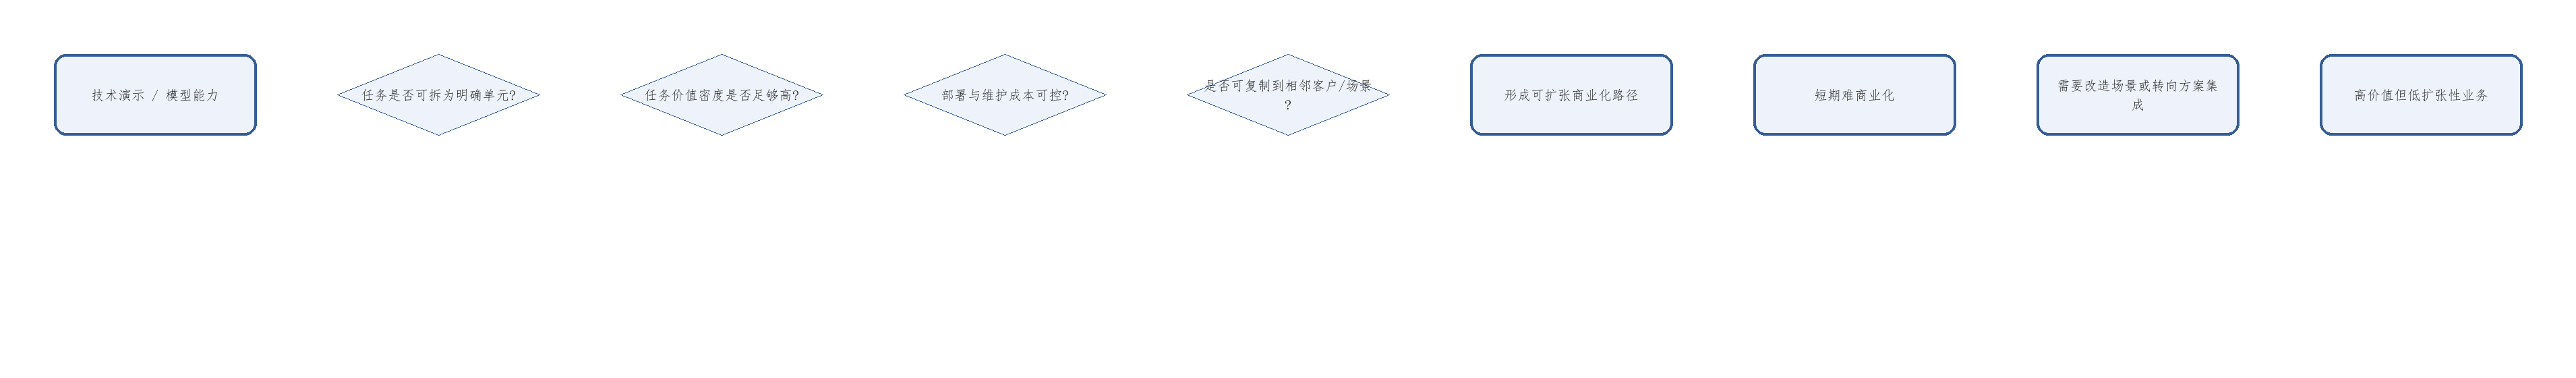
\includegraphics[width=0.9\textwidth,height=0.72\textheight,keepaspectratio]{figures/23-商业化筛选流程图.png}
\caption{23-商业化筛选流程图}
\label{fig:23-商业化筛选流程图}
\end{figure}

\chapter*{表 23-1 典型场景任务单元对照表}
\addcontentsline{toc}{chapter}{表 23-1 典型场景任务单元对照表}
\markboth{表 23-1 典型场景任务单元对照表}{表 23-1 典型场景任务单元对照表}

\begingroup
\small
\begin{xltabular}{\textwidth}{YYYYYYY}
\toprule
场景 & 典型任务单元 & 结构化程度 & 误差容忍度 & 维护难度 & 监管强度 & ROI 可见性 \\
\midrule
\endfirsthead
\toprule
场景 & 典型任务单元 & 结构化程度 & 误差容忍度 & 维护难度 & 监管强度 & ROI 可见性 \\
\midrule
\endhead
制造 & 上下料、工位协作、质检 & 高 & 中 & 中 & 中 & 高 \\
仓储物流 & 分拣、搬运、补货、拣选 & 高 & 中 & 中 & 中 & 高 \\
巡检 & 楼宇/电力/园区巡检 & 中高 & 中 & 中 & 中 & 中高 \\
农业 & 采摘、喷洒、巡田 & 中 & 中 & 高 & 中 & 中 \\
家庭服务 & 收纳、清洁、照护辅助 & 低 & 低 & 高 & 中高 & 低到中 \\
医疗康复 & 辅助操作、康复训练、转运 & 中 & 低 & 高 & 高 & 中 \\
\bottomrule
\end{xltabular}
\endgroup

\chapter*{图表与案例补充}
\addcontentsline{toc}{chapter}{图表与案例补充}
\markboth{图表与案例补充}{图表与案例补充}

本章的图表与案例补充，最重要的不是把场景列得更多，而是把“任务单元 - 约束条件 - 自动化边界 - 商业模式适配”之间的关系固定下来。这样后续新增场景时，就可以直接判断它究竟更接近制造、物流、家庭服务还是高风险环境，而不是每次重新发明一套分类语言。

在长期版本维护中，这一章尤其适合沉淀三类案例。第一类是“先在狭窄场景成功，再逐步扩边界”的正例；第二类是“演示很强但单位经济性始终不闭合”的反例；第三类是“通过人在回路或远程接管先形成业务，再逐步提高自主度”的过渡型案例。只有三类案例并列，商业化章节才不会被单边叙事带偏。

应用落地章节中的图表补充，核心目标是把“商业化判断”从泛泛叙事变成结构化筛选。对具身智能而言，真正决定一个场景能否先跑通的，往往不是展示是否震撼，而是任务结构化程度、误差后果、维护负担和价值密度是否同时满足部署条件。

因此，本章图表不应只是总结性的可视化，而应服务于一个更实用的问题：面对一个新场景时，研究者或分析者应怎样快速判断它更接近“值得进入的商业入口”，还是“更适合作为长期研发目标”。这也是后续版本继续增补行业案例时最值得复用的分析骨架。

在当前版本中，\texttt{\detokenize{图 23-1 商业化筛选流程图}} 已承担“从能力演示到可复制部署”的主流程表达；\texttt{\detokenize{表 23-1 典型场景任务单元对照表}} 则把制造、仓储、巡检、农业、家庭、医疗等场景的误差容忍度、维护难度、监管强度与 ROI 可见性放入统一比较口径。

“值不值得先做”的问题，最终需要被转译成半结构化的 ROI 判断，而不是只停留在定性描述上。23-场景ROI粗估模板 的作用，正是在“人工成本替代、部署改造成本、维护负担、责任风险和复制难度”之间建立统一口径，使场景优先级讨论具备跨版本可更新性。

后续如果要把这一章真正用作季度判断工具，建议同时配合 23-典型场景任务单元对照表 和 23-场景ROI粗估模板 使用。前者负责拆任务单元，后者负责把“值不值得先做”写成统一粗估口径。

若后续更偏向结构化维护，则可以优先使用 23-场景ROI粗估模板-脚本生成版。这样场景字段可以先在 \path{data/processed/场景ROI粗估模板-v0.0.csv} 中修改，再统一导出，避免正文表格和底层字段长期分叉。
